\begin{figure}[h]
    \centering
    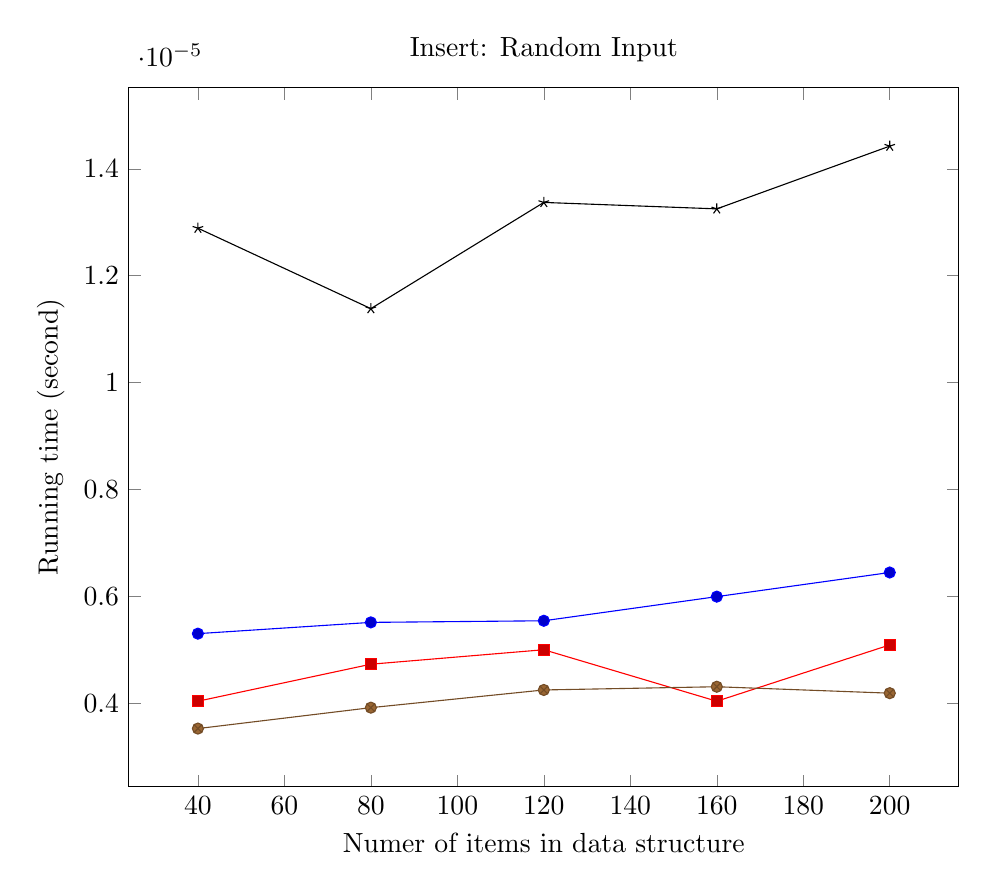
\begin{tikzpicture}
        \begin{axis}[
            xlabel={Numer of items in data structure},
            ylabel={Running time (second)},
            title={Insert: Random Input},
            width=\textwidth
        ]
		\addplot coordinates {
			(200, 6.445152206485671e-06)
			(160, 5.993389201358612e-06)
			(120, 5.541626196228777e-06)
			(80, 5.511508662553455e-06)
			(40, 5.300685926828974e-06)
		};
		\addplot coordinates {
			(200, 5.0898631911044935e-06)
			(160, 4.035749512470988e-06)
			(120, 4.9995105900785266e-06)
			(80, 4.728452787003401e-06)
			(40, 4.035749512473763e-06)
		};
		\addplot coordinates {
			(200, 4.186337180850374e-06)
			(160, 4.306807315548889e-06)
			(120, 4.246572248201019e-06)
			(80, 3.915279377772473e-06)
			(40, 3.523751439996059e-06)
		};
		\addplot coordinates {
			(200, 1.4426298630404455e-05)
			(160, 1.325171481707521e-05)
			(120, 1.3372184951773725e-05)
			(80, 1.1384427729213554e-05)
			(40, 1.2890304412971342e-05)
		};
        \legend{}
        \end{axis}
    \end{tikzpicture}
    \caption{Average of 0 operations, benchmarked every 0, starting at 0.}
\end{figure}